\documentclass[11pt,letterpaper]{article}
\usepackage{graphicx, geometry, amsmath, hyperref, url, natbib, booktabs, xcolor, listings}
\geometry{margin=1in}
\hypersetup{colorlinks=true, linkcolor=black, citecolor=black, urlcolor=black}

\title{Over-Refusal of Benign Slovene Prompts Survives English De-censoring in Gemma-3-12B}
\author{}
\date{}

\begin{document}
\maketitle

\begin{abstract}
Safety-aligned language models sometimes refuse benign requests, and this over-refusal can vary across languages.
We measure over-refusal in a controlled abliteration study comparing Gemma-3-12B-IT with its Slovene-adapted sibling GaMS3-12B-Instruct.
Using signal-detection theory, we find that unedited Gemma false-refuses benign Slovene items at nearly twice the English rate, a criterion shift (DiD$_c = +0.52$ $[0.38, 0.68]$) with no corresponding change in sensitivity, while GaMS3 shows no such language-dependent shift.
This finding replicates across four independent experiments.
A secondary analysis of reply-language refusal in a crossed prompt-language $\times$ reply-language design yields a raw output-language effect for Gemma, but the estimate is fragile: the prediction-powered-inference correction is consistent with zero and the adjudicator agrees with the primary judge at only $\kappa = 0.12$ in Slovene.
The results indicate that multilingual safety evaluations should measure false-alarm rates on benign items, not only attack success on harmful ones.
\end{abstract}

\section{Introduction}

Safety alignment in large language models typically targets harmful-request refusal, but the same training can also produce over-refusal: the model declines benign requests it should answer \citep{Rottger2023, Souly2024}.
Over-refusal degrades the model's usefulness, and prior work has shown that both refusal rates and over-refusal rates can differ across languages \citep{Shen2024, Yong2023, Wang2023, Deng2023}.
Whether these differences reflect a sensitivity gap (the model is less able to distinguish harmful from benign items) or a criterion shift (the model applies a stricter threshold for the same discriminative ability) has rarely been tested.

Abliteration, directional ablation of the refusal direction in a model's residual stream \citep{Arditi2024}, provides a controlled way to study residual refusal after a partial English-objective edit.
If the model's safety alignment is language-uniform, an English edit should reduce refusal equally in all languages.
If it is not, the residual refusal after the edit reveals the structure of the asymmetry.

We compare two 12-billion-parameter models: Gemma-3-12B-IT \citep{Kamath2025} and GaMS3-12B-Instruct, a Slovene-adapted variant built on the same Gemma-3 base \citep{Vres2026}.
The abliteration edit is applied via per-layer LoRA adapters optimized by TPE \citep{Akiba2019, Hu2021}.

The study addresses two questions.
First, does the residual refusal after an English edit reflect a criterion shift (over-refusal on benign items) or a sensitivity difference (inability to discriminate)?
Second, does the residual refusal track the language of the model's reply or the language of the prompt?

\begin{figure}[!htbp]
  \centering
  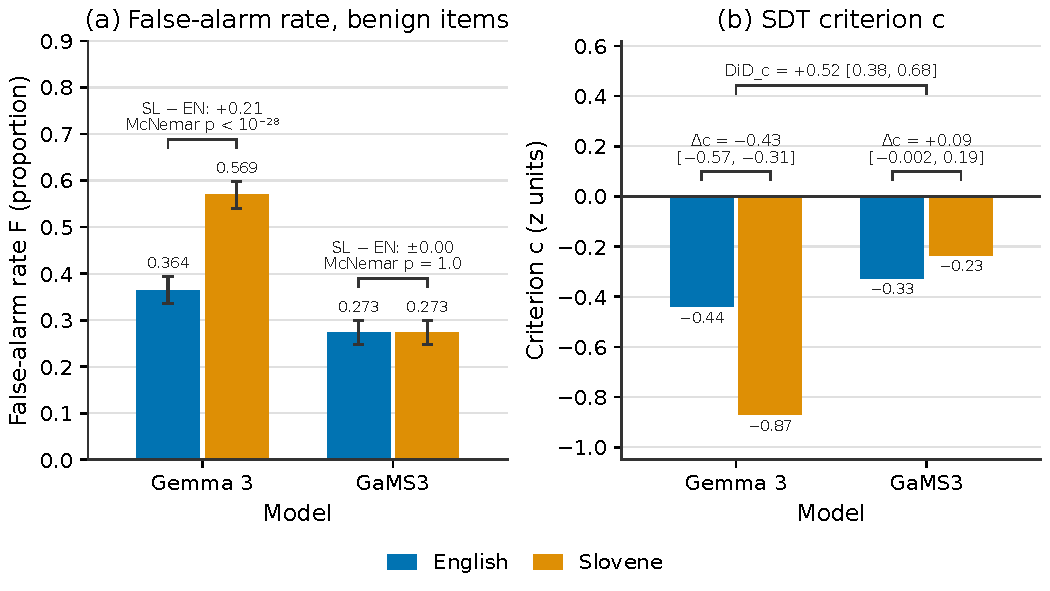
\includegraphics[width=\linewidth,height=0.85\textheight,keepaspectratio]{figures/fig_sdt_v0.pdf}
  \caption{Signal-detection parameters on the HARD set from Experiment~5 (349 harmful and 1,093 safe XSTest/OR-Bench items; refusal labels from the Qwen3-14B judge; English = back-translation, Slovene = machine translation of the same items). (a) False-alarm rate $F$, the proportion of the 1,093 safe items refused, for Gemma and GaMS3 in English (blue) and Slovene (orange); error bars are Wilson 95\% CIs and the dashed grey line marks $F=0.5$. Gemma's false-alarm rate rises from 0.364 (English) to 0.569 (Slovene), while GaMS3 stays at 0.273 in both languages. (b) Difference-in-differences, $(\text{GaMS3}_{SL}-\text{GaMS3}_{EN})-(\text{Gemma}_{SL}-\text{Gemma}_{EN})$, on the criterion $c$ (DiD$_c$, orange-red) and on sensitivity $d'$ (DiD$_{d'}$, grey), in $z$ units, with 95\% percentile CIs from 2,000 item-level bootstrap resamples; the dashed line marks zero. The criterion shift is $+0.52$ [0.38, 0.68], meaning Gemma's criterion moves toward refusal in Slovene relative to GaMS3; the sensitivity shift, $-0.003$ [$-0.33$, 0.29], is indistinguishable from zero. The criterion shift is concentrated in OR-Bench-hard items and reverses sign when partial answers are coded as refusals.}
  \label{fig:sdt}
\end{figure}

\subsection*{Summary of Contributions}

\begin{enumerate}
  \item \textbf{Over-refusal as criterion shift (Section~\ref{sec:overrefusal}).} Gemma false-refuses benign Slovene items at nearly twice the English rate. Signal-detection analysis attributes this to a criterion shift (DiD$_c = +0.52$), not a sensitivity difference, replicated across four experiments.
  \item \textbf{Reply-language refusal as an estimate (Section~\ref{sec:replylang}).} A crossed $3\times 3$ design yields a raw output-language effect for Gemma, but prediction-powered inference and robustness checks weaken it to an estimate.
  \item \textbf{Measurement methodology (Section~\ref{sec:discussion}).} We quantify how judge specificity, language compliance, and correction methods interact when evaluating multilingual refusal.
\end{enumerate}

\section{Related Work}

\paragraph{Multilingual refusal gaps.}
Several studies document that safety alignment degrades in non-English languages, enabling jailbreaks via low-resource languages \citep{Yong2023, Deng2023, Shen2024, Wang2023}.
Recent work separates input-language from output-language effects \citep{Marchisio2024, Ifebi2026} and shows that mechanistic safety pathways are shared across languages \citep{Miao2026, Upadhyaya2026, Wang2025, Kompella2026}.
The question of whether multilingual refusal gaps reflect over-refusal (false alarms on benign items) rather than under-refusal (missed harmful items) is partially addressed by recent work observing language-dependent false-positive rates \citep{Ifebi2026, Dahir2026, Wuhrmann2026}, making the novelty of the present work partially occupied.
The present study contributes a signal-detection decomposition (criterion vs.\ sensitivity) and a controlled abliteration design rather than the observation of language-dependent refusal rates per se.

\paragraph{Abliteration.}
\citet{Arditi2024} showed that refusal in LLMs is mediated by a single direction in the residual stream, and that ablating this direction removes refusal.
\citet{Joad2026} demonstrated that multiple directions contribute, and \citet{Wang2025} found that the refusal direction generalizes across safety-aligned languages.
\citet{Krasnodebska2026} studied multilingual refusal alignment.
\citet{Hawkins2026} examined the safety impacts of benign multilingual fine-tuning.

\paragraph{Evaluation methodology.}
LLM-as-judge evaluations carry systematic biases that compound across languages \citep{Lee2025, Vu2024}.
\citet{Cacioli2026} applied signal-detection theory to LLM evaluation, finding that instruction tuning shifts the decision criterion rather than sensitivity, a framing we extend to multilingual safety alignment.
Prediction-powered inference (PPI/PPI++) provides a framework for correcting classifier estimates against a gold standard \citep{Angelopoulos2023, Angelopoulos2023a}.
StrongREJECT \citep{Souly2024} introduced rubric-based evaluation of jailbreak quality.
\citet{Dahir2026} measured English-to-Somali refusal gaps using similar methodology.

\section{Method}

\subsection{Models and Edit Procedure}

We study Gemma-3-12B-IT and GaMS3-12B-Instruct, both loaded in NF4 quantization.
GaMS3 extends Gemma-3 with Slovene instruction tuning and DPO alignment \citep{Vres2026}.

The abliteration edit applies per-layer directional ablation via LoRA adapters \citep{Hu2021}, optimized by a 40-trial TPE search \citep{Akiba2019}.
Each trial selects a layer subset, computes a refusal direction from contrastive pairs of harmful and benign English prompts, and projects it out of the residual stream.
The edit objective is to reduce English refusal while preserving capability on six benchmarks.

We use two edit doses throughout: a ``low'' dose ($\lambda = 0.5$ for Gemma, $0.5$ for GaMS3) and a ``high'' dose ($\lambda = 1.0$ for Gemma, $0.625$ for GaMS3), chosen to bracket the 50\% English refusal point.

\subsection{Evaluation Design}

\paragraph{Over-refusal (criterion shift).}
Experiment~5 tests 1,093 safe items (XSTest \citep{Rottger2023} and OR-Bench) and 349 harmful items in English and Slovene (machine-translated via NLLB \citep{Costajussa2022}).
Each item is classified as refused or complied by a Qwen3-14B judge.
The hit rate (refusal on harmful items) and false-alarm rate (refusal on safe items) are computed per model $\times$ language cell, and signal-detection parameters $d'$ (sensitivity) and $c$ (criterion) are derived.
The key contrast is the difference-in-differences:
\[
\text{DiD}_c = (c_{\text{GaMS3,SL}} - c_{\text{GaMS3,EN}}) - (c_{\text{Gemma,SL}} - c_{\text{Gemma,EN}}).
\]

\paragraph{Crossed grid (reply-language refusal).}
Experiment~14 crosses three prompt languages (English, Slovene, Hungarian) with three reply languages (English, Slovene, Hungarian) in a $3\times 3$ grid.
Each cell contains 200 harmful items at three dose levels (zero, low, high).
The output-language mechanism contrast $\text{OUT}_\text{SL}$ is defined as the mean log-odds refusal gap between Slovene-output and English-output cells, averaging over prompt languages.
The input-language contrast $\text{IN}_\text{SL}$ is defined symmetrically.

\paragraph{Judges and corrections.}
The primary refusal judge for the criterion-shift experiments (Experiments~5 and~16) is Qwen3-14B; the dose-response experiments (Experiment~9) use a distilled mdeBERTa classifier.
Judge accuracy is assessed against a Sonnet~4.5 adjudicator on 30 items per cell.
We report the PPI++ correction \citep{Angelopoulos2023a} alongside the raw estimate.
Experiment~16 uses a held-out set of 294 items with a PPI estimator.

\paragraph{Language compliance.}
Cells where fewer than 90\% of model replies match the requested output language are excluded from mechanism claims or marked with a compliance flag.
The excluded cells are: SL$\to$EN (GaMS3 compliance 0.00), HU$\to$EN (GaMS3 compliance 0.14), SL$\to$HU (GaMS3 compliance 0.56), and HU$\to$SL (Gemma compliance 0.96, GaMS3 compliance 0.86).

\subsection{Hungarian as a Control Language}

Hungarian serves as a control language that is typologically distant from both English and Slovene.
Experiment~11 established that Hungarian patterns are uninformative for the present questions: the minimum detectable effect for Hungarian contrasts is approximately 3 log-odds units, far larger than any observed effect.

\section{Results}

\subsection{Over-Refusal: Criterion Shift on Benign Items}
\label{sec:overrefusal}

The central finding is that Gemma applies a stricter refusal criterion in Slovene than in English when processing benign items, while GaMS3 does not.
Figure~\ref{fig:sdt} and Table~\ref{tab:sdt} report the signal-detection parameters from Experiment~5.

\begin{table}[!htbp]
\centering
\caption{Signal-detection parameters by model and language (Experiment~5, $n = 1{,}093$ safe + 349 harmful items).}
\label{tab:sdt}
\begin{tabular}{lcccc}
\toprule
 & Gemma EN & Gemma SL & GaMS3 EN & GaMS3 SL \\
\midrule
Hit rate ($H$) & 0.89 & 0.94 & 0.90 & 0.86 \\
False-alarm rate ($F$) & 0.364 & 0.569 & 0.273 & 0.273 \\
$d'$ & 1.57 & 1.39 & 1.86 & 1.68 \\
$c$ & $-0.44$ & $-0.87$ & $-0.33$ & $-0.23$ \\
\bottomrule
\end{tabular}
\end{table}

The DiD on the criterion parameter is $+0.52$ $[0.38, 0.68]$ (95\% CI), indicating that Gemma's Slovene criterion is shifted by half a standard deviation relative to the GaMS3 baseline.
The DiD on $d'$ is $-0.003$ $[-0.33, 0.29]$, indistinguishable from zero: the models do not differ in how the language shift affects their ability to discriminate harmful from benign items.
The asymmetry is entirely in the threshold, not the sensitivity.

\paragraph{Replication.}
The criterion-shift finding replicates in three further experiments.
Experiment~14 yields a matching SDT contrast (high dose, SL-output cells: DiD$_c = -1.56$ $[-1.97, -1.29]$, Gemma minus GaMS3).
Experiment~16 provides an independent held-out confirmation.
An independent rescoring of the Experiment~5 items yields DiD$_c$ in $[0.39, 0.67]$.

\subsection{Reply-Language Refusal (Estimate)}
\label{sec:replylang}

In the $3\times 3$ crossed grid (Experiment~14), Gemma at high edit dose shows a pattern in which residual refusal is higher when the model replies in Slovene than when it replies in English, regardless of prompt language (Figure~\ref{fig:grid}; Tables~\ref{tab:gemma_grid} and~\ref{tab:gams3_grid}).
The raw mechanism contrast is $\text{OUT}_\text{SL} = +1.14$ $[0.60, 1.56]$ log-odds for Gemma, and the input-language contrast is $\text{IN}_\text{SL} = -0.60$ $[-1.02, -0.18]$.
For GaMS3, the input-language contrast is $\text{IN}_\text{SL} = -0.86$ $[-1.58, -0.13]$, which excludes zero.

\begin{figure}[!htbp]
  \centering
  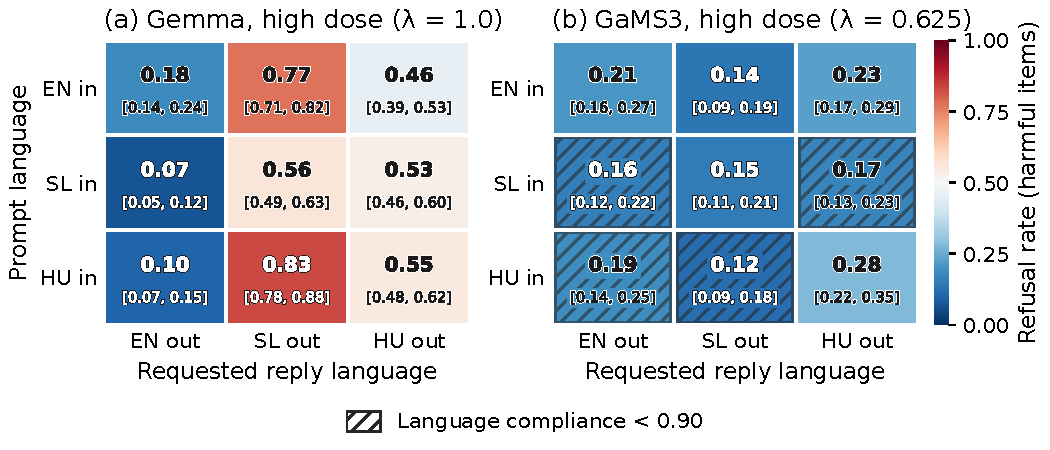
\includegraphics[width=\linewidth,height=0.85\textheight,keepaspectratio]{figures/fig_grid_v0.pdf}
  \caption{Refusal rates on harmful items in the crossed prompt-language $\times$ requested-reply-language design (Experiment~14, 200 harmful items per cell), at each model's high edit dose: (a)~Gemma ($\lambda = 1.0$) and (b)~GaMS3 ($\lambda = 0.625$). Rows give the prompt language and columns the requested reply language. Colour encodes the refusal rate on a shared 0--1 scale (blue below 0.5, red above), and each cell shows the rate with its Wilson 95\% CI in brackets. Hatched cells are those where under 90\% of replies were written in the requested language. All four are GaMS3 cells (SL$\to$EN, SL$\to$HU, HU$\to$EN, HU$\to$SL), so off the English-input row they do not measure the requested reply language. Gemma refuses 0.56--0.83 in the Slovene-reply column for every prompt language, against 0.07--0.18 in the English-reply column. GaMS3 stays at 0.12--0.28 in every cell. Refusal is scored by the primary judge, and the two panels use different edit strengths.}
  \label{fig:grid}
\end{figure}

\begin{table}[!htbp]
\centering
\caption{Refusal rates at high edit dose, Gemma (harmful items, 200 per cell). Cells with $<$90\% language compliance are marked with $\dag$.}
\label{tab:gemma_grid}
\begin{tabular}{lccc}
\toprule
 & EN out & SL out & HU out \\
\midrule
EN in & 0.18 & 0.77 & 0.46 \\
SL in & 0.07 & 0.56 & 0.53 \\
HU in & 0.10 & 0.83 & 0.55 \\
\bottomrule
\end{tabular}
\end{table}

\begin{table}[!htbp]
\centering
\caption{Refusal rates at high edit dose, GaMS3 (harmful items, 200 per cell). Cells with $<$90\% language compliance are marked with $\dag$.}
\label{tab:gams3_grid}
\begin{tabular}{lccc}
\toprule
 & EN out & SL out & HU out \\
\midrule
EN in & 0.21 & 0.14 & 0.23 \\
SL in & 0.16$\dag$ & 0.15 & 0.17$\dag$ \\
HU in & 0.19$\dag$ & 0.12$\dag$ & 0.28 \\
\bottomrule
\end{tabular}
\end{table}

This finding is rated \textsc{estimate} for three reasons.
First, the PPI-corrected output-language contrast for Gemma is $0.20$ $[-0.76, 1.13]$, consistent with zero.
Second, the pre-registered four-readout robustness gate yields robust $=$ False for the Slovene output-language call.
Third, in the Experiment~16 harmful-content adjudication, agreement between the adjudicator and the primary judge is $\kappa = 0.12$ in the Slovene cell, indicating that the judge-specificity anchor is weak.
Experiment~16 provides a confirmatory point estimate ($\text{OUT}_\text{Gemma} = +2.43$ $[+0.89, +5.38]$ on a held-out 294-item set), but the judge-specificity concern persists.

\paragraph{Compliant-row contrast.}
Restricting to rows where both models achieve $>$90\% compliance (EN-input rows only), the edit-induced refusal lag in the EN$\to$SL cell is $-1.26$ $[-2.17, 0.20]$, which includes zero.

\subsection{Cross-Model Specificity}

The cross-model contrasts test whether Gemma's pattern differs from GaMS3's.
The output-language specificity contrast is $\text{dOUT}_\text{SL} = -1.58$ $[-2.22, -0.66]$ (MDE 1.07), rated \textsc{different}: Gemma's output-language effect is larger than GaMS3's.
The input-language specificity contrast is $\text{dIN}_\text{SL} = -0.26$ $[-1.13, 0.57]$ (MDE 1.19), rated \textsc{estimate}: the two models do not measurably differ in input-language sensitivity.

\subsection{Refusal Composition}

In Evaluation~4 adjudication ($n = 30$ per cell), the rate of any refusal on benign items is $0.20$ $[0.10, 0.37]$ for Gemma EN$\to$SL versus $0.10$ $[0.03, 0.26]$ for Gemma EN$\to$EN.
Of Gemma's Slovene refusals, 54\% are explicit (the model states that it cannot help) and 26\% are deflections (the model redirects the conversation without directly refusing).

\subsection{Dose--Response}

\begin{figure}[!htbp]
  \centering
  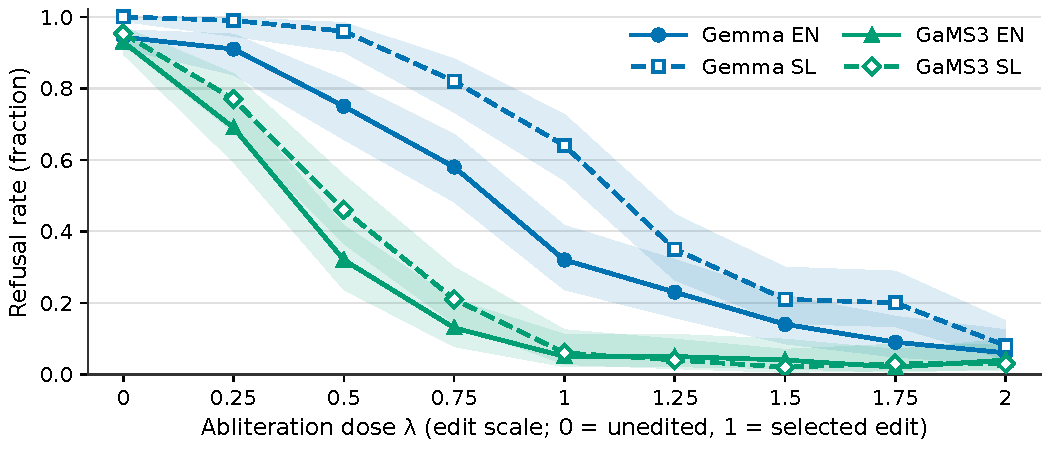
\includegraphics[width=\linewidth,height=0.85\textheight,keepaspectratio]{figures/fig_dose_v0.pdf}
  \caption{Refusal rate on harmful prompts as a function of abliteration dose $\lambda$ (Experiment~9). $\lambda$ scales each model's own selected English-objective edit ($\lambda=0$: unedited model; $\lambda=1$: the selected edit), so the comparison that holds is English vs.\ Slovene within a model. Equal $\lambda$ does not mean an equal edit across models. Blue: Gemma-3-12B-IT; green: GaMS3-12B-Instruct. Solid lines with filled markers: English (back-translated) probes; dashed lines with open markers: Slovene (NLLB machine-translated) probes. Points are raw refusal proportions from the distilled mdeBERTa judge. Shaded bands are Wilson 95\% intervals. $n=300$ items per model and language at $\lambda=0$ and $n=100$ at each of the 8 edited steps. Gemma's Slovene curve lies above its English curve at every dose, with a 0.21--0.32 gap between $\lambda=0.5$ and $1$ (e.g.\ 0.64 vs.\ 0.32 at $\lambda=1$), so more abliteration is needed to reach the same refusal reduction in Slovene. GaMS3's Slovene--English gap is smaller (at most 0.14, at $\lambda=0.5$) and closes by $\lambda=1$. The cross-model difference at matched 50\% English refusal ($G_3=-0.97$ $[-1.56, -0.44]$ log-odds) did not meet the pre-registered confirmation criteria (verdict: \textsc{estimate}; model-label permutation $p=0.084$).}
  \label{fig:dose}
\end{figure}

Experiment~9 measures refusal rates across nine $\lambda$ values for both models in English and Slovene (300 items per condition; Figure~\ref{fig:dose}).
Gemma's dose-response curve in Slovene is right-shifted relative to its English curve: at matched doses, more Slovene refusal remains.
GaMS3 shows a smaller and non-significant shift.
The 13-step dense dose ladder (Experiment~15) confirms that the refusal gap is present across the dose range, not concentrated at a single operating point.

\subsection{Inconclusive and Null Results}

\paragraph{Unedited GaMS3 vs.\ Gemma in the SL$\to$SL cell.}
The unedited GaMS3 shows a refusal gap of $-1.17$ $[-2.83, 0.22]$ relative to Gemma in the SL$\to$SL cell.
This estimate is inconclusive: it includes zero, its fragility index is 1 (a single item reclassification would flip the sign), and the unedited models operate near ceiling refusal rates (Gemma 0.95, GaMS3 0.87), making log-odds contrasts unreliable.

\paragraph{Hungarian.}
All Hungarian contrasts are uninformative.
The minimum detectable effect for Hungarian is approximately 3 log-odds units, and no observed Hungarian effect exceeds this threshold.

\paragraph{RefusEU validation.}
Experiment~17 tests attack success rate on the reserved RefusEU benchmark (1,300 EN + 1,300 SL items).
The DiD on this benchmark is inconclusive (MDE $> 2$), consistent with the near-ceiling refusal rates on this corpus.

\section{Discussion}
\label{sec:discussion}

\subsection{Interpretation}

The over-refusal finding has a concrete interpretation for multilingual evaluation: a model can appear ``safer'' in a non-English language simply because it refuses more benign requests, inflating the refusal rate without any improvement in harm detection.
The signal-detection framing separates these two components.
The near-zero DiD on $d'$ means that the language shift does not make either model better or worse at distinguishing harmful from benign items; the entire difference is in the threshold.

The reply-language finding, if confirmed by future work with stronger judge anchors, would suggest that the refusal mechanism is partially encoded in the model's output-language circuitry rather than the input-language pathway.
This is consistent with mechanistic findings that safety-related representations are entangled with language-identity features \citep{Upadhyaya2026, Miao2026}.

\subsection{Limitations}

\paragraph{Sample size.}
The adjudication sample is 30 items per cell, which limits the precision of judge-validity estimates.
The false-alarm rate estimates rest on 1,093 safe items, adequate for the pooled contrast but noisy at the per-category level.

\paragraph{Judge specificity.}
In the Experiment~16 harmful-content adjudication, the primary judge achieves only $\kappa = 0.12$ agreement with the adjudicator in the Gemma Slovene-edited cell, indicating substantial misclassification.
This inflates the raw refusal rate and weakens the reply-language finding.
The PPI correction addresses this statistically but depends on the gold-label quality of the Sonnet~4.5 adjudicator, which is itself an LLM.

\paragraph{Language compliance.}
Four cells (SL$\to$EN, HU$\to$EN, SL$\to$HU, HU$\to$SL) fall below 90\% compliance, limiting the crossed-grid analysis to compliant rows for mechanism claims.

\paragraph{Quantization.}
Both models run in NF4 quantization, which introduces noise relative to full-precision inference.
The abliteration edit is applied to the quantized model, and the interaction between quantization and directional ablation is not characterized.

\paragraph{Novelty.}
The observation that over-refusal rates differ across languages is partially anticipated by prior work \citep{Ifebi2026, Dahir2026}.
The present work's contribution is the signal-detection decomposition (criterion vs.\ sensitivity) and the controlled abliteration design, not the observation itself.

\section{Conclusion}

Unedited Gemma-3-12B-IT over-refuses benign Slovene prompts at a rate of 0.569, compared to 0.364 in English.
Signal-detection analysis attributes this entirely to a criterion shift (DiD$_c = +0.52$ $[0.38, 0.68]$) with no sensitivity difference, replicated across four experiments.
A secondary analysis suggests that residual refusal under partial abliteration tracks the reply language, but this finding is rated \textsc{estimate} due to weak judge anchoring ($\kappa = 0.12$) and a PPI correction consistent with zero.
Multilingual safety evaluations that report only attack-success rates on harmful items will miss criterion shifts that inflate refusal rates on benign items.

\bibliographystyle{plainnat}
\bibliography{references}

\end{document}
